\def\QRCODE{TB_image_TUT.IMG.cornea_fourier_pythonqrcode.png}
\def\QRPAGE{http://www.iptutorials.science/tree/master/TB_image/TUT.IMG.cornea_fourier/python}
\pcorrectionsection{Python correction}

\begin{python}
import numpy as np
from scipy import misc, ndimage #read/write images
import matplotlib.pyplot as plt # plots
\end{python}

\subsection{Introduction and utilities} To display a spectrum, the following function can be useful:
\begin{python}
# Displays spectrum and phase in an image (grayscale)
def viewSpectrumPhase(amplitude, phase):
    plt.figure()
    plt.subplot(1,2,1)
    plt.imshow(np.log(1+amplitude), plt.cm.gray);
    
    plt.subplot(1,2,2)
    mmax = np.max(phase);
    mmin = np.min(phase);
    if (mmax == mmin):
        B=0;
    else:
        B = 255*(phase-mmin)/(mmax-mmin);
        
    plt.imshow(B, cmap=plt.cm.gray);

\end{python}

\subsection{Fourier transform}
Results (amplitude and phase) are represented in Fig. \ref{fig:fourier:python:cornee}.

\begin{python}
cornea = imageio.imread('cornee.png')
print type(cornea)
print cornea.shape, cornea.dtype

plt.subplot(131)
plt.imshow(cornea, cmap=plt.cm.gray)
\end{python}

\begin{python}
## Fourier transform
#  result is complex
#  fftshift is used by convention the get frequency 0 at center of image
spectre = np.fft.fftshift(np.fft.fft2(cornea));

A = abs(spectre);
G = np.angle(spectre);

viewSpectrumPhase(A, G);
\end{python}


\subsection{Inverse Fourier Transform}

\begin{python}
## inverse Fourier transform
cornee2 = np.real(np.fft.ifft2(np.fft.fftshift(spectre)));
plt.figure()
plt.imshow(cornee2, cmap=plt.cm.gray);
plt.title('inverse FT');
\end{python}

The Fourier transform, although very powerful, is really difficult to interpret in 2D. The main information is not contained in the amplitude, but in the phase. The following reconstructions will illustrate it (see Fig.\ref{fig:partial}).

\begin{python}
## inverse Fourier transform, without the phase
cornee_amplitude=  np.real(np.fft.ifft2(np.fft.fftshift(A)));
plt.figure();
plt.imshow(cornee_amplitude, cmap=plt.cm.gray);
plt.title('inverse FT on amplitude');
\end{python}

\begin{python}
## inverse Fourier transform on phase only
complex_phase = np.exp(1j*G);
cornee_phase=np.real(np.fft.ifft2(np.fft.fftshift(complex_phase)));
plt.figure()
plt.imshow(cornee_phase, cmap=plt.cm.gray);
plt.title('inverse FT on phase');
\end{python}

\begin{figure}[htbp]
 \centering\caption{Reconstruction of partial informations (phase or amplitude only).}%
 \subfloat[Reconstruction with amplitude only.]{
\includegraphics[width=.45\linewidth]{sansphase.png}}\hfill
 \subfloat[Reconstruction with phase only.]{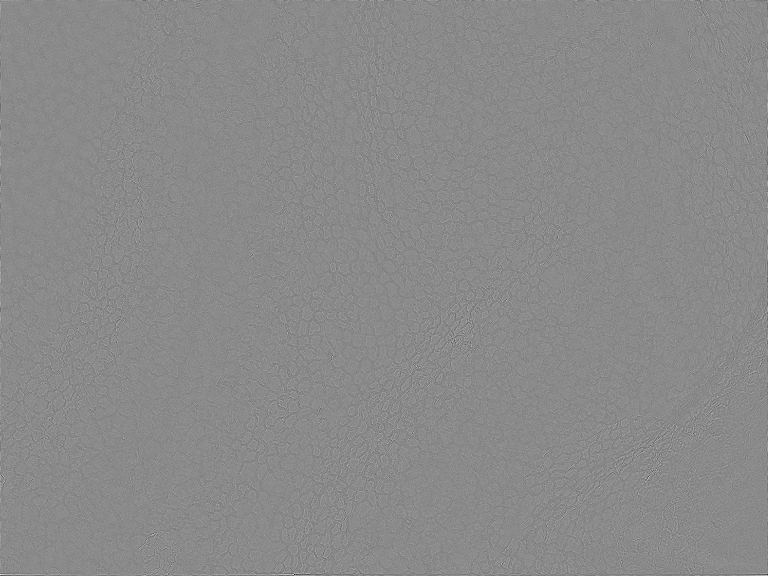
\includegraphics[width=.45\linewidth]{phase.png}}%
 \label{fig:partial}%
\end{figure}


\subsection{Low-pass and high-pass filtering}
The results are illustrated in Fig. \ref{fig:fourier:python:filters}. Two functions are defined.


A low pass-filter consists in the suppression of values for frequencies lower than a cut-off frequency.

\begin{figure}[H]
	\centering\caption{Fourier basic filtering of cornea image.}%
	\subfloat[High Pass filter.]{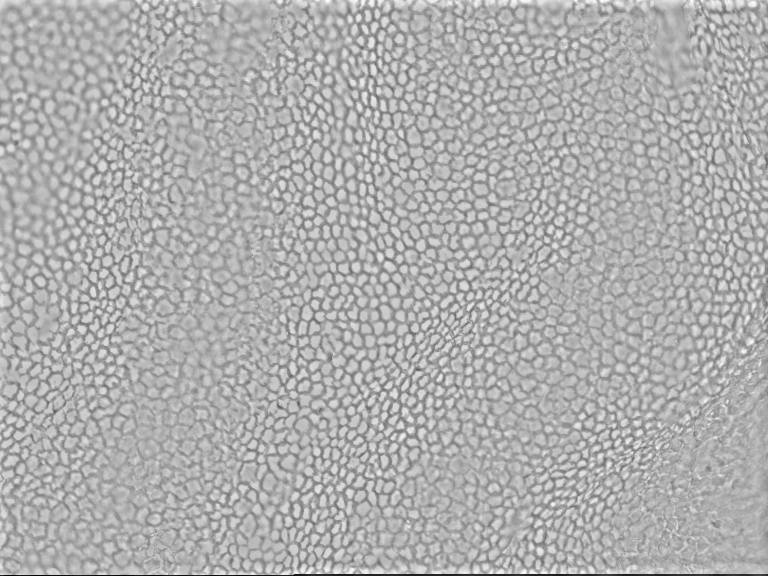
\includegraphics[width=.45\linewidth]{corneaHP.png}}
	\hfill
	\subfloat[Low Pass filter.]{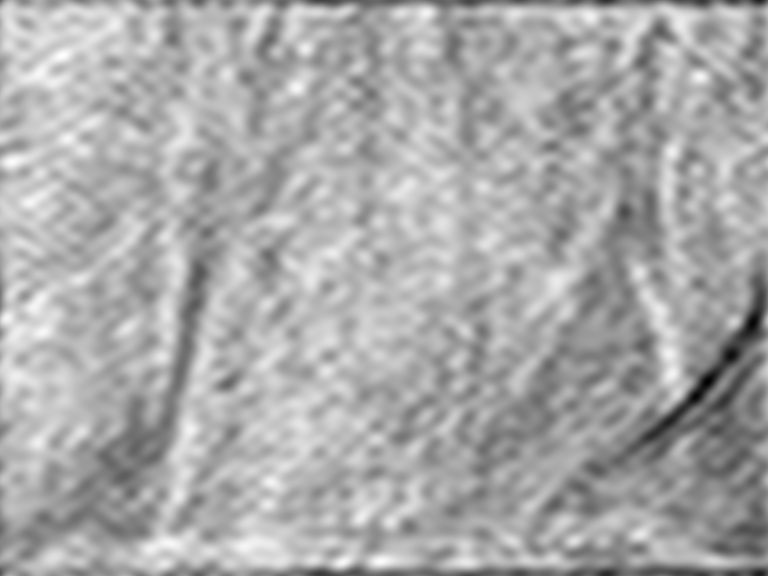
\includegraphics[width=.45\linewidth]{corneaLP.png}}%
	\label{fig:fourier:python:filters}%
\end{figure}

 \begin{python} 
def LowPassFilter(spectrum, cut):
    """Low pass filter of the FFT (spectrum)
    The shape of this filter is a square. fftshift has been applied so that 
    frequency 0 lays at center of spectrum image
    @param spectrum: FFT2 transform
    @param cut     : cut value of filter (no physical unit, only number of pixels)
    """
    X,Y = spectrum.shape;
    mask = np.zeros((X,Y), "int");
    mx = X/2; my = Y/2;
    mask[mx-cut:mx+cut, my-cut:my+cut] = 1;
    f = spectrum * mask;
    plt.figure
    plt.imshow(abs(f)); plt.title('Low pass filter')
    return f;
\end{python}

A high pass filter is exactly the opposite: suppression of the values under the cut-off frequency.
\begin{python}
def HighPassFilter(spectrum, cut):
    """High pass filter of the FFT (spectrum)
    The shape of this filter is a square. fftshift has been applied so that 
    frequency 0 lays at center of spectrum image
    @param spectrum: FFT2 transform
    @param cut     : cut value of filter (no physical unit, only number of pixels)
    """
    X,Y = spectrum.shape;
    mask = np.ones((X,Y), "int");
    mx = X/2; my = Y/2;
    mask[mx-cut:mx+cut, my-cut:my+cut] = 0;
    f = spectrum * mask;
    plt.figure
    plt.imshow(abs(f)); plt.title('High pass filter')
    return f;
\end{python}


In the following application, the image is loaded and the effects of a low-pass and high-pass filters are illustrated.
\begin{python}
# FT of original image
cornea = imageio.imread('cornee.png')
spectre = np.fft.fftshift(np.fft.fft2(cornea));
# low pass filter
L = LowPassFilter(spectre, 30)
viewSpectrumPhase(abs(L), np.angle(L))
corneaLP = np.real(np.fft.ifft2(np.fft.fftshift(L)))
# high pass filter
H = HighPassFilter(spectre, 30)
viewSpectrumPhase(abs(H), np.angle(H))
corneaHP = np.real(np.fft.ifft2(np.fft.fftshift(H)))
# display results and filters
plt.figure();
plt.subplot(1,2,1)
plt.imshow(corneaLP, plt.cm.gray);plt.title('reconstruction after LP filtering')
plt.subplot(1,2,2)
plt.imshow(corneaHP, plt.cm.gray);plt.title('reconstruction after HP filtering')
 \end{python}

\vspace*{-5pt}
\subsection{Application: evaluation of cellular density}
The cells can be considered as a pattern, and its frequency repetition can found in the Fourier transform. More precisions on this application can be found in \cite{Ruggeri2005,Grisan2005,Ruggeri2007,Selig2015} on the relation between the real cellular density and the image pixels.

\begin{python}
cornea = imageio.imread('cornee.tif')
# Fourier Transform
spectre = np.fft.fftshift(np.fft.fft2(cornea));
amplitude = abs(spectre);
# Filter amplitude
Blurred = ndimage.filters.gaussian_filter(amplitude, 5);
plt.figure
plt.subplot(1,2,1); 
plt.imshow(np.log(1+Blurred), plt.cm.gray); 
plt.title('filtered amplitude')
# Observe frequency peaks
plt.subplot(1,2,2);
plt.plot(np.log(1+Blurred[:,Y/2])); 
plt.title('peak observation and cells frequency')
 \end{python}

 The results are illustrated in Fig. \ref{fig:fourier:python:cornee}.\vspace*{-5pt}
 \begin{figure}[htbp]
 \centering\caption{The two peaks represent the frequency of repetition of the cellular pattern, i.e. it can be used to compute the cellular density.}%
  \subfloat[Amplitude of Fourier Transform.]{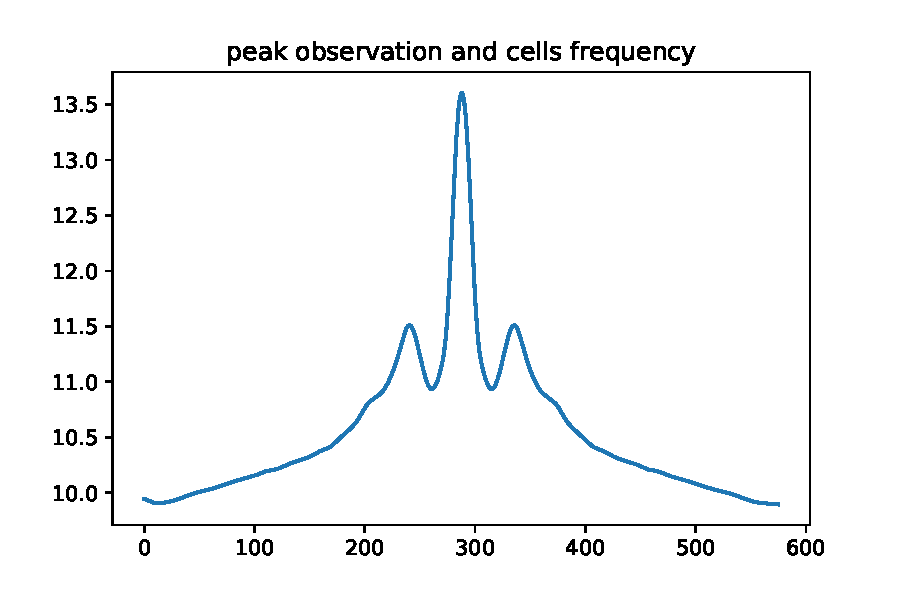
\includegraphics[width=.45\linewidth]{analyse_cornee.pdf}}\hspace{1cm}
  \subfloat[Filtering of amplitude.]{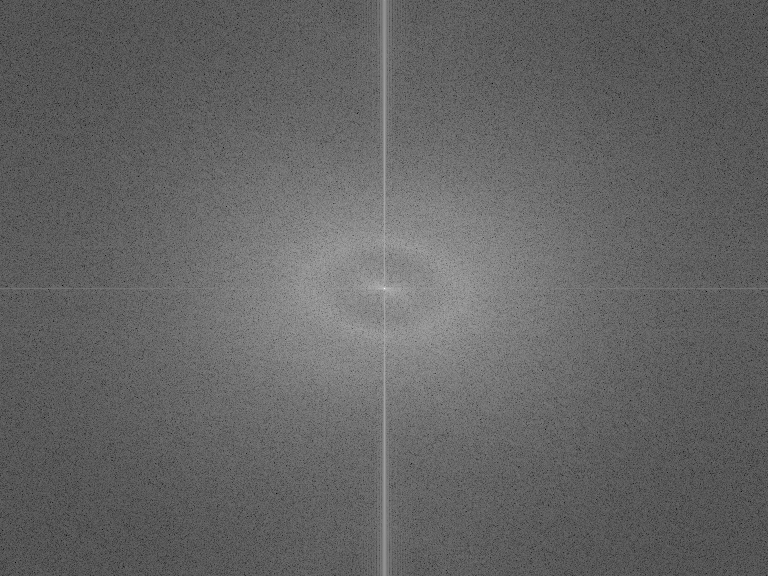
\includegraphics[width=.38\linewidth]{amplitude.png}}%
  \label{fig:fourier:python:cornee}\vspace*{-10pt}%
 \end{figure}
